%% Preambel
\documentclass[conference,compsoc,final,a4paper,12pt]{IEEEtran}
\usepackage[utf8]{inputenx}

\newcommand{\autoren}[0]{Ahmed Salame, Ida Vanessa Gouleu Mokam}

\newcommand{\dokumententitel}[0]{Websockets mit Grails}

% Hie muss normalerweise nichts angepasst werden
\usepackage[pdftex]{graphicx}
\graphicspath{{img/}}
\DeclareGraphicsExtensions{.pdf,.jpeg,.png}
\usepackage[cmex10]{amsmath}
\usepackage{algorithmic}
\usepackage{array}
\usepackage{dblfloatfix}
\usepackage{url}
\usepackage[autostyle=true,german=quotes]{csquotes}
\usepackage[backend=biber]{biblatex}
\usepackage{booktabs}
\usepackage{xcolor}
\usepackage{listings}             % Source Code listings
\usepackage[printonlyused]{acronym}

% Farben definieren
\definecolor{linkblue}{RGB}{0, 0, 100}
\definecolor{linkblack}{RGB}{0, 0, 0}
\definecolor{darkgreen}{RGB}{14, 144, 102}
\definecolor{darkblue}{RGB}{0,0,168}
\definecolor{darkred}{RGB}{128,0,0}
\definecolor{comment}{RGB}{63, 127, 95}
\definecolor{javadoccomment}{RGB}{63, 95, 191}
\definecolor{keyword}{RGB}{108, 0, 67}
\definecolor{type}{RGB}{0, 0, 0}
\definecolor{method}{RGB}{0, 0, 0}
\definecolor{variable}{RGB}{0, 0, 0}
\definecolor{literal}{RGB}{31,0, 255}
\definecolor{operator}{RGB}{0, 0, 0}

\usepackage[ngerman]{betababel}
\usepackage[
	    unicode=true,
      hypertexnames=false,
      colorlinks=true,
      colorlinks=false,
      linkcolor=darkblue,
      citecolor=darkblue,
      urlcolor=darkblue,
      pdftex
   ]{hyperref}
%	 \PrerenderUnicode{ü}

% Einstellungen für Quelltexte
\lstset{
      xleftmargin=0.1cm,
      basicstyle=\scriptsize\ttfamily,
      keywordstyle=\color{keyword},
      identifierstyle=\color{variable},
      commentstyle=\color{comment},
      stringstyle=\color{literal},
      tabsize=2,
      lineskip={2pt},
      columns=flexible,
      inputencoding=utf8,
      captionpos=b,
      breakautoindent=true,
	  breakindent=2em,
	  breaklines=true,
	  prebreak=,
	  postbreak=,
      numbers=none,
      numberstyle=\tiny,
      showspaces=false,      % Keine Leerzeichensymbole
      showtabs=false,        % Keine Tabsymbole
      showstringspaces=false,% Leerzeichen in Strings
      morecomment=[s][\color{javadoccomment}]{/**}{*/},
      literate={Ö}{{\"O}}1 {Ä}{{\"A}}1 {Ü}{{\"U}}1 {ß}{{\ss}}2 {ü}{{\"u}}1 {ä}{{\"a}}1 {ö}{{\"o}}1
}

\hypersetup{
  pdftitle={\dokumententitel},
	pdfauthor={\autoren},
	pdfdisplaydoctitle=true
}

% Wo liegt Sourcecode?
\newcommand{\srcloc}{src/}

% Literatur einbinden
\addbibresource{literatur.bib}

\begin{document}

% Titel des Dokuments
\title{\dokumententitel}

% Namen der Autoren
\author{
  \IEEEauthorblockN{\autoren}
  \IEEEauthorblockA{
    Hochschule Mannheim\\
    Fakultät für Informatik\\
    Paul-Wittsack-Str. 10,
    68163 Mannheim
    }
}

% Titel erzeugen
\maketitle
\thispagestyle{plain}
\pagestyle{plain}
 % Weitere Einstellungen aus einer anderen Datei lesen

% Eigentliches Dokument beginnt hier
% ----------------------------------------------------------------------------------------------------------

% Kurze Zusammenfassung des Dokuments
\begin{abstract}
Dieses Paper soll aufzeigen, wie Websockets mit Grails realisiert werden kann. Zunächst wird auf einige Grundlagen näher eingegangen, um dem Leser ein Besseres Verständnis für das Thema zu vermitteln. 

--TODO--
\end{abstract}

\tableofcontents

\section{Einleitung}
 
WebSockets \ref{websocket} sind eine langlebige, interaktive, Zwei-Wege-Kanal Kommunikation zwischen einem Client-Browser und End-Server, die kontinuierliche Kommunikation ohne Abfragen ermöglichen. WebSockets sind schon seit einigen Jahren da, seit sie von RFC 6455 vorgeschlagen wurden und so ziemlich alle großen Browser haben seitdem Unterstützung gewonnen. 

Spring \ref{spring}, das Java-MVC-Framework, erhielt die integrierte WebSocket-Unterstützung in Version 4.0, und diese Unterstützung wurde seitdem in Spring Boot und Grails integriert (Grails-Unterstützung wird von diesem hilfreichen Plugin bereitgestellt). Dieser Artikel gibt einen Überblick über einige Beispiele, um sich mit WebSockets vertraut zu machen und gleichzeitig etwas über dessen Integration in Grails zu lernen, als Grails Version 3.0 erreichte.
 
\section{Forschungsmethode}

Beim Recherchieren wurde unter anderem Google Books\footnote{https://books.google.de/} verwendet, um passende Literatur zu finden. Des weiteren wurde die Homepage The Groovy Project herangezogen, um die Sprache Groovy näher zu beleuchten.
Zudem wurde nach passenden Quellen aus dem Internet gesucht, um bestimmte Themen näher zu erläutern. Zudem sind diese auch für jeden zugänglich. 

\section{State of the art}

Wenn Clients den Server regelmäßig in einem bestimmten Zeitfenster abfragen, nur um zu fragen, ob aktualisierte Informationen verfügbar sind, kann es zu Problemen kommen. Wenn sich viele Clients gleichzeitig mit dem Server verbinden, kann der Thread-Pool des Servers erschöpft sein, wodurch die Anwendung angehalten wird.

Es gibt zwar nicht blockierende Server auf dem Markt, aber oft können Sie Ihr Serverprodukt nicht einfach wechseln oder die gesamte Anwendungsarchitektur in eine Nachrichten gesteuerte Architektur ändern.

Eine mögliche architektonische Lösung war daher das Konzept von WebSockets.
Die HTML5 Websocket-Spezifikation definiert eine bidirektionale Duplexkommunikation zwischen Client und Server über eine einzige Verbindung. Zwei-Wege-Kommunikation bedeutet, dass ein Server mit WebSockets eine Nachricht an seine Clients senden kann. Folglich kann ein gegebener Thread-Server mehr Clients bedienen oder mehr gleichzeitige Verbindungen unterstützen.

WebSocket ist keine Socket-Technik, wie man es von einem Unix-System kennt, WebSocket ist ein Protokoll. Der WebSocket startet als gewöhnliche HTTP-Verbindung (http: //), fragt dann aber den Server, ob er zum WebSocket-Protokoll (ws: //) wechseln möchte. Wenn diese Anforderung erteilt wird, wird die HTTP-Verbindung unterbrochen und durch eine WebSocket-Verbindung über dieselbe zugrunde liegende TCP / IP-Verbindung ersetzt. Der WebSocket verwendet Port 80 oder 443. Nun können die Kommunikationspakete zwischen Client und Server hin- und hergeschickt werden. Sie reisen sogar durch Proxies und Firewalls, was die Anwendungsentwicklung erheblich erleichtert.

\section{Ein Beispiel von WebSockets mit Grails}

Dieser Demonstrator sendet die CPU-Last des Servers an den Webbrowser eines Clients. Auf der Serverseite existiert ein Dienst SimpleMessagingService, der die CPU-Last alle 5 Sekunden misst. Das Ergebnis wird in eine Themenwarteschlange "topic / cpuLoad" gestellt. Über das WebSocket-Protokoll wird der Inhalt der Warteschlange an die Browser aller Clients übermittelt, die diese Themenwarteschlange abonniert haben. Alle abonnierten Browser werden alle gleichzeitig aktualisiert. Abbildung \ref{cpuausl} zeigt dieses Beispiel.

\begin{figure*}[h]
  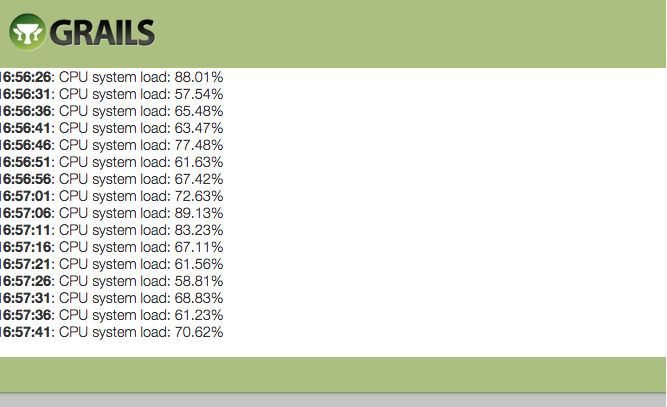
\includegraphics[width=\textwidth,height=7cm]{websocketbrowser.png}
  \caption{Ausgabe der CPU Auslastung mit Grails\protect\footnotemark}
  \label{cpuausl}
\end{figure*}
\footnotetext{https://jolorenz.wordpress.com/2015/07/21/websockets-with-grails/}%s%s

Ein sehr nettes WebSocket-Plugin existiert für Grails. Es erleichtert die Integration der Spring 4.0 WebSocket-Unterstützung. Fügen Sie einfach compile ": spring-websocket: 1.3.0" zum Plugins-Bereich von Grails BuildConfig.groovy hinzu.
Mit Spring 4.0 WebSocket gibt es verschiedene Möglichkeiten, Nachrichten zu senden oder zu empfangen. Hier werde ich das SimpMessagingTemplate und seine convertAndSend-Funktion verwenden.

\begin{lstlisting}[language=Groovy,caption={SimpMessagingTemplate.java}, label=listingGb]
package com.jolorenz
 
import org.springframework.messaging.simp.SimpMessagingTemplate
import java.lang.management.ManagementFactory;
 
import com.sun.management.OperatingSystemMXBean;
import grails.transaction.Transactional
import groovy.json.JsonBuilder
 
@Transactional
class SimpleMessageService {
 
   SimpMessagingTemplate brokerMessagingTemplate
   OperatingSystemMXBean bean = (com.sun.management.OperatingSystemMXBean)   
   ManagementFactory.getOperatingSystemMXBean()
 
   void systemCpuLoad() {
 
      def cpuLoad = bean.getSystemCpuLoad()
      cpuLoad = (cpuLoad*100).round(2)
 
      def builder = new JsonBuilder()
      builder {
         message("CPU system load: " + cpuLoad + "%")
         timestamp(new Date())
      }
      def msg = builder.toString()
      brokerMessagingTemplate.convertAndSend "/topic/cpuLoad", msg
   }
}
\end{lstlisting}

Als nächstes benötigen wir eine HTML / Javascript-Seite mit der entsprechenden Themenwarteschlange, z. "/ Topic / cpuLoad".

\begin{lstlisting}[language=HTML,caption={Beispiel einer GSP Datei}, label=listingGb]
&lt;!DOCTYPE html&gt;;
&lt;html&gt;;
   &lt;head&gt;;
   &lt;meta name="layout" content="main" /&gt;
   &lt;asset:stylesheet src="application.css" /&gt;
   &lt;asset:javascript src="application.js" /&gt;
   &lt;asset:javascript src="jquery" /&gt;
   &lt;asset:javascript src="spring-websocket" /&gt;
 
   &lt;script type="text/javascript"&gt;
      $(function() { 
         //Create a new SockJS socket - this is what connects to the server
         //(preferably using WebSockets).
         var socket = new SockJS("${createLink(uri: '/stomp')}");
 
         //Build a Stomp client to send messages over the socket we built.
         var client = Stomp.over(socket);
 
         //Have SockJS connect to the server.
         client.connect({}, function() {             
            client.subscribe("/topic/cpuLoad", function(message) {
               var msg = JSON.parse(message.body)
               var time = '&lt;strong&gt;;' + new Date(msg.timestamp).toLocaleTimeString() + '&lt;/strong&gt;'
               $("#cpuLoadDiv").append(time + ': ' + msg.message + "&lt;br/&gt;");
            });
         });                
      });
   &lt;/script&gt; 
&lt;/head&gt;
 
&lt;body&gt;
   &lt;div id="cpuLoadDiv"&gt;&lt;/div&gt;
&lt;/body&gt;
&lt;/html&gt;
\end{lstlisting}

Das ist alles was benötigt wird, um eine WebSocket-Kommunikation zwischen Server und Client einzurichten. Es ist ein einfaches Beispiel und es fehlen Funktionen wie Filter für Benutzergruppen oder Sicherheit, aber es gibt eine Idee, sich mit WebSockets vertraut zu machen.
Was sind die Nachteile?

WebSocket ist eine Browserfunktion und nicht alle Browser unterstützen diese Funktion. Wahrscheinlich werden in naher Zukunft alle Browser und Server WebSockets unterstützen.
CanIUse bietet einen guten Überblick über die unterstützten Webbrowser.

\section{Einleitung}

\section{Weiterer Titel}

\section{Fazit}

%--------------------------

\lstlistoflistings

\listoffigures

\section*{Abkürzungen}
\addcontentsline{toc}{section}{Abkürzungen}

\begin{acronym}
\acro{POJO}{Plain Old Java Object}
\acro{GSP}{Groovy Server Pages}
\acro{JTA}{Java Transaction API}
\acro{JSR}{Java Specification Request}
\acro{JVM}{Java Virtual Machine}
\acro{URI}{Uniform Resource Identifier}
\end{acronym}

% Literaturverzeichnis
\addcontentsline{toc}{section}{Literatur}
\printbibliography

\end{document}